%Tex-Stuff
\documentclass[a4paper,12pt]{article}

%Imports
\usepackage[pdftex]{graphicx}
\usepackage[utf8]{inputenc}
\usepackage{subcaption}
\usepackage{hyperref}
%\usepackage{enumitem}


%%%%%%%%%%%%%%%%%%%%%%%%%%%%%%%%%%%%%%%%%%%%%%%%
\begin{document}

\section{PaperOverflow: Produktivision}
Die Beschreibung der Produktvision erfolgt noch den Feldern des  \href{http://www.romanpichler.com/tools/vision-board/}{"Product-Vision-Boards"} von Roman Pichler. 
\begin{figure}[h!]
  \centering
  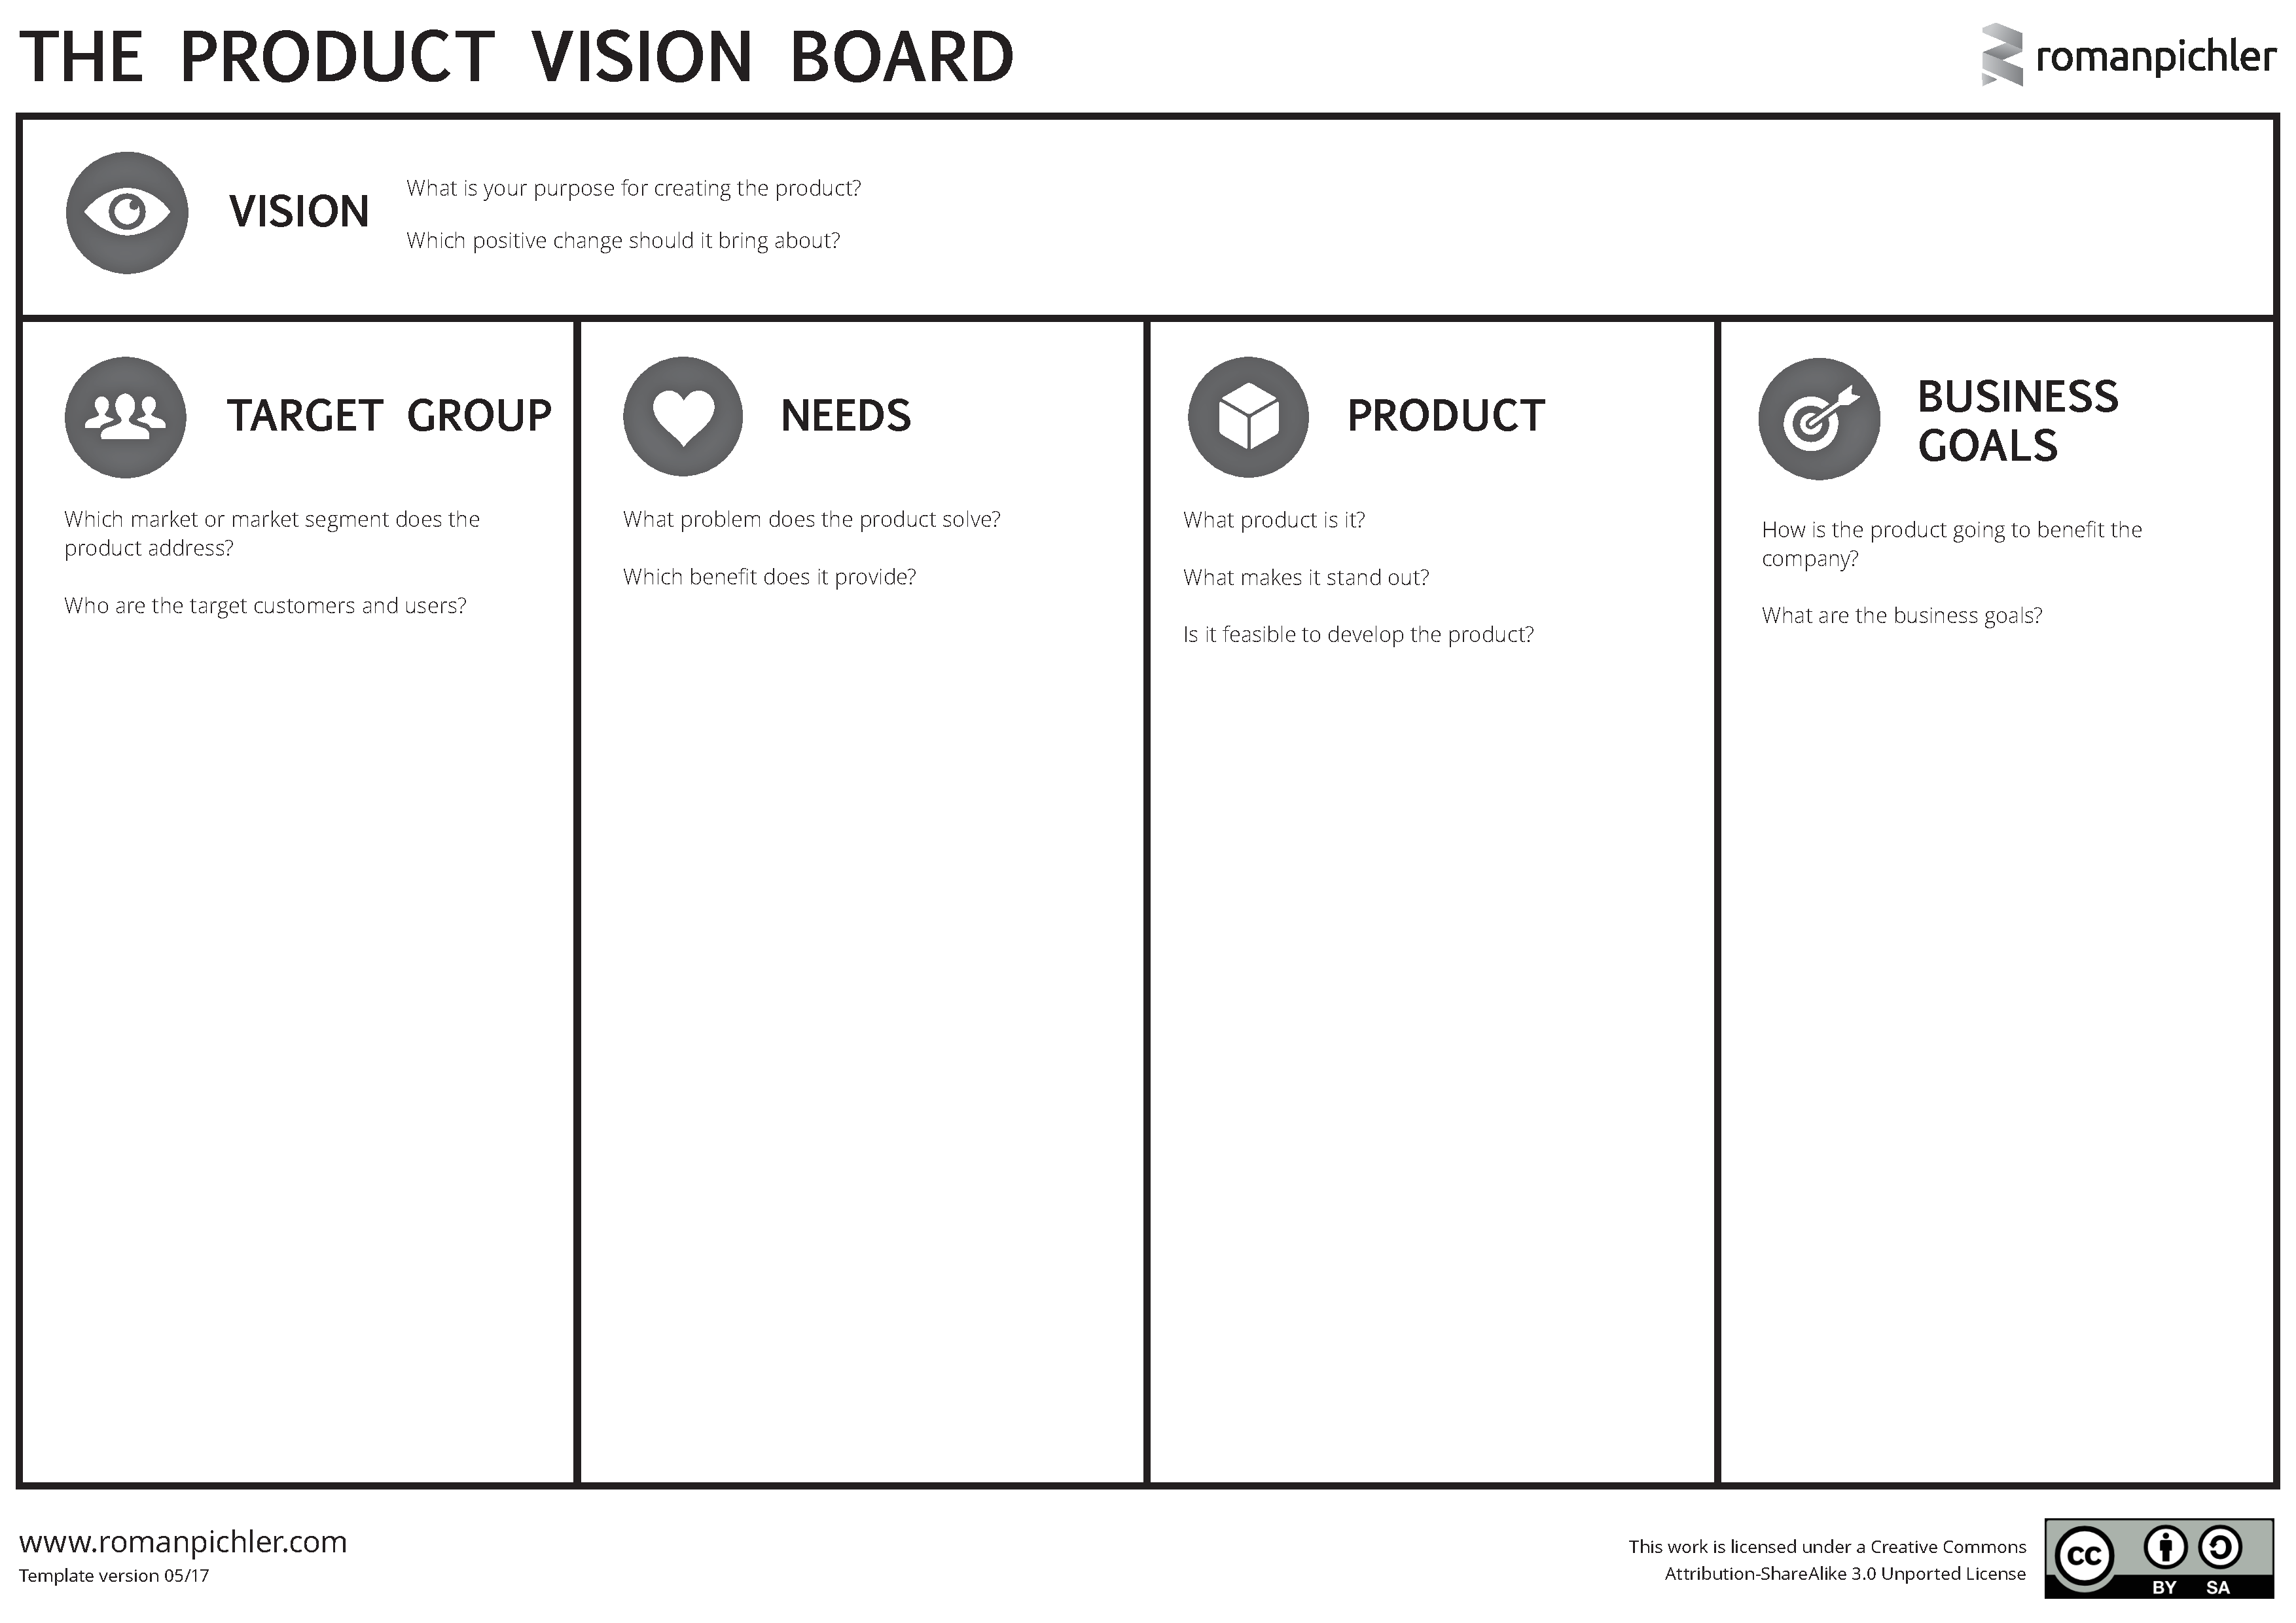
\includegraphics[width=0.7\linewidth]{res/PVB.pdf}
\end{figure}

Besonderes Augenmerk soll dabei auf die Produktbeschreibung gelegt werden.
Die Geschäfts-Ziele hingegen, sollen aufgrund der geringen Relevanz für das Projekt nicht beleuchtet werden.

\subsection{Vision}
Ziel von PaperOverflow ist es den Autoren von wissenschaftlichen Arbeiten im Bereich der Literaturverwaltung zu unterstützen. Dabei soll die PaperOverflow im Gegensatz zu ähnlichen Produkten komfortabel und unkompliziert sein, fehlerhafte Zitate vermeiden, ein Aufsuchen von zitierbaren Textstellen ermöglichen und mit wachsender Menge an zu verwaltenden Dokumenten besser werden.

\subsection{Zielgruppe}
Wer sind die Anwender von PaperOverflow?\\
Zunächst wird PaperOverflow von Benutzern verwendet, deren Ziel es ist eine wissenschaftliche Arbeit zu verfassen. PaperOverflow soll für diese Benutzer die Verwaltung von wissenschaftlichen Veröffentlichungen anderer Autoren übernehmen.\\
Vorrangig soll das Auditorium von PaperOverflow aus Anwendern bestehen, welche zum Verfassen der Wissenschaftlichen Arbeit LaTeX verwenden. Jedoch sollen auch Nicht-LaTeX-Benutzer PaperOverflow zur Verwaltung von Veröffentlichungen nutzen können.\\
PaperOverflow soll zum einen von Benutzern verwendet werden, die technisch versiert sind und gerne mit komplexer wirkenden, dafür jedoch mächtigeren Oberflächen arbeiten. Zum anderen sollen auch weniger technisch versierte Nutzer durch eine einfache Oberfläche angenehm mit PaperOverflow arbeiten können.\\
Des Weiteren werden die Anwender von PaperOverflow verscheiden große Mengen an Veröffentlichungen zu verwalten haben. Dabei soll sich der Einsatz der Software schon ab wenigen Dokumenten lohnen, aber auch riesige Mengen an Veröffentlichungen handhaben können. Das Verhältnis, welche Dokumente in digitaler Form vorliegen und welche als haptisches Exemplar vorhanden sind, variiert dabei ebenfalls von Nutzer zu Nutzer.\\
\\
Um die oben genannten variierenden Eigenschaften der Zielgruppe zu veranschaulichen, sollen als Vertreter der gesamten Zielgruppe drei Personas aufgelistet werden.

\paragraph{Wolfgang der Word-User mit wenigen Dokumenten}
- Wolfgang möchte einen kurzen wissenschaftlichen Artikel veröffentlichen und hat sich entscheiden dies in Microsoft Word zu tun. Er benötigt nur eine Hand voll wissenschaftlicher Quellen, die er richtig zitiert. Diese Quellen liegen ihm teils digital, teils analog vor. Er ist nicht weiter technisch versiert und es ist auch nicht zu erwarten, dass er in näherer Zeit weitere wissenschaftliche Arbeiten schreiben wird.

\paragraph{Larissa die LaTeX-Userin mit vorrangig digitalen Dokumenten}
- Larissa nutzt LaTeX, um ihre Abschlussarbeit anzufertigen. Sie setzt sich dafür zum ersten Mal intensiver mit LaTeX und BibTeX auseinander. Sie hat für Ihre Arbeit etwa 40 potentielle Quellen, von denen Sie voraussichtlich etwa 30 zitieren wird. Die Quellen liegen Larissa hauptsächlich in digitaler Form vor.

\paragraph{Prof. Probst der LaTeX-Power-User mit vorrangig analogen Dokumenten}
- Prof. Probst ist LaTeX-Vollprofi und verfasst regelmäßig wissenschaftliche Dokuemnte zu verschiedenen Themen und verschiedenen Fachrichtungen. Er hat inzwischen eine Dokumentensammlung von 1200 wissenschaftlichen Veröffentlichungen. Davon stehen die meisten in seinem Bücherregal, nur wenige liegen ihm in digitaler Form vor.

\subsection{Bedürfnisse}
\begin{itemize}
\item Komfortables hinzufügen von Literaturquellen
\item Überblick behalten. $\to$ Komfortables verwalten von Literaturquellen
\item Angenehmes Suchen, schnelles finden von guten Zitaten, Komfort-Funktionen.
\item Zum Zitat in wenigen Klicks.
\item Sicherstellen von Einhaltung der Zitierstandards
\item Komfortabel weiterverarbeitbar $\to$ quick an dirty oder für langfristige Nutzung
\item Ordnung über digitale Dokumente behalten.
\end{itemize}

\subsection{Produktbeschreibung}

Sie haben sich dazu entschieden eine wissenschaftliche Arbeit zu verfassen und sind nun dabei sich Wissen zum Themengebiet heranzuziehen? Und der Haufen der Veröffentlichungen wir immer größer und größer? Und ganz allmählich unbezwingbar? Sie nähern sich langsam der Grenze, ab der sie einfach nicht mehr Dokumente handhaben können? Dem Overflow an Papers? 
\begin{center}
Keine Panik! 
\end{center}
Der Overflow ist nicht böse, er braucht nur die richtige Handhabe. Mit PaperOverflow holen Sie das Maximum aus Ihrer Dokumentensammlung heraus!\\ \\
PaperOverflow unterstützt Sie in Ihrem Arbeiten, in den drei folgenden Schritten:

\renewcommand\thesubfigure{\arabic{subfigure}}
\begin{figure}[h!]
  \centering
  \begin{subfigure}[b]{0.32\linewidth}
    
\includegraphics[width=\linewidth]{res/step1.png}
    \caption{Den PaperOverflow nähren.}
    %\label{fig:1} 
  \end{subfigure}
  \begin{subfigure}[b]{0.32\linewidth}
    
\includegraphics[width=\linewidth]{res/step2.png}
    \caption{Den PaperOverflow durchsuchen}
    %\label{fig:2} 
  \end{subfigure}
  \begin{subfigure}[b]{0.32\linewidth}
    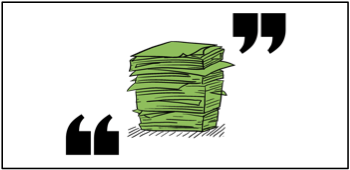
\includegraphics[width=\linewidth]{res/step3.png}
    \caption{Den PaperOverflow zitieren}
    %\label{fig:3} 
  \end{subfigure}
\end{figure}



\paragraph{Den PaperOverflow nähren.}\

PaperOverflow unterstützt Sie bei dem Erfassen Ihrer Dokumente. \\

\textbf{Print-Exemplare:}
\begin{itemize}
	\item Buch im Schrank
	\item Erfassn über ISBN oder Titel oder Autor mit Auto-Vervollständigung.
	\item Dann holt PaperOverflow Vorschläge. Nur kurze Sichtprüfung ggf. Auswahl Alternativvorschläge. Mit wenigen Klicks Buch erfasst.
	\item Einige Stichworte automatisch erfasst. Stichworte mit wenigen Klicks hinzufügbar.
\end{itemize} \

\textbf{Als Datei:}
\begin{itemize}
	\item Drag it, Drop it!
	\item Alles an einer Stelle: Diese legt PaperOverflow für Sie ab. Auf bedarf wieder als Datei exportierbar.
	\item Keine Arbeit: Holt die Meta-Informationen: Nur Sicht-Prüfungen und Auswahl Alternativvorschläge.
	\item Einige Stichworte automatisch erfasst. Stichworte mit wenigen Klicks hinzufügbar.
\end{itemize}\ 

\textbf{Mehr als eine große Halte?}
\begin{itemize}
	\item Ordnung von Beginn an: Verscheidene Kategorien anlegbar 
	\item Einfaches Hinzufügen zu Literatursammlung -> Schon da optional wählbar
	\item Nachher auch sortierbar
\end{itemize}

Alles zusammen schön übersichtlich.
Sie sind technisch versiert, lesen BibteX fließend und möchten mehr sehen? Schalten Sie um auf den wiss mod!
\\
\paragraph{Den PaperOverflow durchsuchen}\

Dann sitzen Sie da und suchen nach guten Stellen.
\begin{itemize}
	\item Auto-Vervollständigung bei Suche
	\item Komfortabel Suchen in Stichworten, Abstract, Titeln, Autoren. (iTunes)
	\item erhalten Sie Vorschläge für ähnliche Dokumente
	\item historisierte Suchanfragen
\end{itemize}

Das Dokument liegt digital vor? Zeigen Sie es an und lesen Sie rein!

\paragraph{Den PaperOverflow zitieren}\ 

Passendes Zitat in Ihrem Overflow gefunden? \\

\textbf{Zitieren Sie!} 
\begin{itemize}
	\item In Dokument gleich mit Zeilenangabe
	\item aber auch für print-Exemplare schnell angegeben.
\end{itemize}

\textbf{Set bauen}
\begin{itemize}
	\item QuickQuote: Mit einem Klick haben Sie den entsprechenden BibTex in der Zwischenablage und können Ihn weiterverarbeiten.
	\item Oder: Zu Zitaten hizufügen und weitersuchen.
	\item Dabei: Info hizufügen.
	\item Sie haben mehr als eine Arbeit, für die Sie zitate sammeln? Legen Sie Zitat-Sets an!
\end{itemize}

\textbf{Export!}
\begin{itemize}
	\item Sets rausgeben in gängigen Exportformaten: ...
	\item Export als Referenzlisten: ..
	\item Zusammenarbeit mit anderen? Per Mail senden: Zitat, Refliste.
\end{itemize}

%\pagebreak

\end{document}
%%%%%%%%%%%%%%%%%%%%%%%%%%%%%%%%%%%%%%%%%%%%%%%%